%  qd.tex
%  
%  This work was supported by the Director, Office of Science, Division
%  of Mathematical, Information, and Computational Sciences of the
%  U.S. Department of Energy under contract number DE-AC03-76SF00098.
%
%  (C) September 2000-2004
\documentclass[11pt]{article}
\usepackage{graphicx}
\usepackage{amsthm}

\pagestyle{plain}

\setlength{\textwidth}{6.5in}
\setlength{\textheight}{8.5in}
\setlength{\topmargin}{-0.2in}
\setlength{\oddsidemargin}{0.0in}
\setlength{\evensidemargin}{0.0in}

% All thm/def/lem/etc... have same numbering
\newtheorem{thm}{Theorem}
\newtheorem{defn}[thm]{Definition}
\newtheorem{lem}[thm]{Lemma}
\newtheorem{prop}[thm]{Proposition}

\theoremstyle{definition}
\newtheorem{alg}[thm]{Algorithm}

\newcommand{\round}{\mathrm{round}}
\newcommand{\fl}{\mathrm{fl}}
\newcommand{\err}{\mathrm{err}}
\newcommand{\ulp}{\mathrm{ulp}}
\newcommand{\hi}{\mathrm{hi}}
\newcommand{\lo}{\mathrm{lo}}
\newcommand{\eps}{\varepsilon}
\newcommand{\epsqd}{\varepsilon_\mathrm{qd}}


\title{Library for Double-Double and Quad-Double Arithmetic\footnotemark[1]}
\author{Yozo Hida\footnotemark[2] \and Xiaoye S. Li\footnotemark[3]
  \and David H. Bailey\footnotemark[3]}
\date{\today}

\begin{document}
\maketitle

% change foot note symbols
\renewcommand{\thefootnote}{\fnsymbol{footnote}}

\footnotetext[1]{This research was supported by the Director, 
  Office of Science, Division of Mathematical, Information, and
  Computational Sciences of the U.S. Department of Energy under 
  contract number DE-AC03-76SF00098.}
\footnotetext[2]{Computer Science Division, University of California, 
  Berkeley, CA 94720 ({\tt yozo@cs.berkeley.edu}).}
\footnotetext[3]{NERSC, Lawrence Berkeley National Laboratory, 1 Cycloton Rd, 
  Berkeley, CA 94720 ({\tt xiaoye@nersc.gov}, {\tt dhbailey@lbl.gov}).}

% change footnote symbols back to numbers
\renewcommand{\thefootnote}{\arabic{footnote}}

\vspace{1cm}
\begin{abstract}
  A double-double number is an unevaluated sum of two IEEE double 
  precision numbers, capable of representing at least 106 bits of 
  significand.   Similarly, a quad-double number is an unevaluated sum of 
  four IEEE double precision numbers, capable of representing at least 
  212 bits of significand.  Algorithms for various arithmetic operations 
  (including the four basic operations and various algebraic and 
  transcendental operations) are presented. A C++ implementation of 
  these algorithms is also described, along with its C and Fortran 
  interfaces.  Performance of the library is also discussed.
\end{abstract}

\newpage
\tableofcontents
\newpage

\section{Introduction} \label{sec:intro}
Multiprecision computation has a variety of application areas, such as
pure mathematics, study of mathematical constants, cryptography,
and computational geometry. Because of this, many arbitrary precision 
algorithms and libraries have been developed using only the fixed
precision arithmetic. They can be divided into two groups based on
the way precision numbers are represented. Some libraries store numbers in a
{\em multiple-digit} format, with a sequence of digits coupled with a 
single exponent, such as the symbolic computation package
Mathematica, Bailey's MPFUN~\cite{bai-mp}, Brent's MP~\cite{brent} and
GNU MP~\cite{gnu-mp}.  An alternative approach is to store numbers
in a {\em multiple-component} format, where a number is expressed
as unevaluated sums of ordinary floating-point words, each with its own
significand and exponent.  Examples of this format 
include~\cite{dek71,pri92,she97}.  The multiple-digit approach can 
represent a much larger range of numbers, whereas the multiple-component 
approach has the advantage in speed.

We note that many applications would get full benefit from using merely
a small multiple of (such as twice or quadruple) the working precision,
without the need for arbitrary precision.
The algorithms for this kind of ``fixed'' precision can be made
significantly faster than those for arbitrary precision.
Bailey~\cite{bai-dd} and Briggs~\cite{kbriggs97} have developed
algorithms and software for ``double-double'' precision, twice the 
double precision. They used the multiple-component format, where a 
double-double number is represented as an unevaluated
sum of a leading double and a trailing double.

In this paper we present the algorithms used in the {\tt qd} library, 
which implements both double-double and quad-double arithmetic.
A quad-double number is an unevaluated sum of four IEEE doubles.
The quad-double number $(a_0, a_1, a_2, a_3)$ represents the exact
sum $a = a_0 + a_1 + a_2 + a_3$, where $a_0$ is the most sigficant component.
We have designed and implemented algorithms for basic arithmetic
operations, as well as some algebraic and transcendental functions.
We have performed extensive correctness tests and compared the results 
with arbitrary precision package MPFUN.
Our quad-precision library is available at
{\tt http://www.nersc.gov/\~{ }dhbailey/mpdist/mpdist.html}.
Our quad-double library has been successfully integrated into a parallel 
vortex roll-up simulation code; this is briefly described in
\cite{hida00}.  

The rest of the paper is organized as follows.
Section~\ref{sec:prelim} describes some basic properties of IEEE
floating point arithmetic and building blocks for our quad-double
algorithms. In Section~\ref{sec:basic} we present the quad-double
algorithms for basic operations, including renormization, addition,
multiplication and division.
Section~\ref{sec:algebraic} and~\ref{sec:transcendental}
present the algorithms for some algebraic operations and transcendental
functions. Section~\ref{sec:misc} describes some auxiliary functions.
Section~\ref{sec:implement} briefly describes our C++ library 
implementing the above algorithms.
Section~\ref{sec:performance} presents the timing results of the
kernel operations on different architectures.
Section~\ref{sec:future} discusses future work.

\section{Preliminaries} \label{sec:prelim}
In this section, we present some basic properties and algorithms of IEEE 
floating point arithmetic used in quad-double arithmetic.
These results are based on Dekker \cite{dek71}, Knuth \cite{knu81}, 
Priest \cite{pri92}, Shewchuk \cite{she97}, and others.  In fact, 
many of the algorithms and diagrams are directly taken from, or based on, 
Shewchuk's paper.

All basic arithmetics are assumed to be performed in IEEE double format, 
with round-to-even rounding on ties.  For any binary operator 
$\cdot \in \{+, -, \times, /\}$, we use $\fl(a \cdot b) = a \odot b$ to denote
the floating point result of $a \cdot b$, and define $\err(a \cdot b)$
as $a \cdot b = \fl(a \cdot b) + \err(a \cdot b)$.
Throughout this paper, $\eps = 2^{-53}$ is the machine epsilon for
IEEE double precision numbers, and $\epsqd = 2^{-211}$ is
the precision one expects for quad-double numbers.

\begin{lem} {\rm \cite[p. 310]{she97}}
  Let $a$ and $b$ be two $p$-bit floating point numbers such that
  $|a| \ge |b|$.  Then $|\err(a+b)| \le |b| \le |a|$.
\end{lem}

\begin{lem} {\rm \cite[p. 311]{she97}}
  Let $a$ and $b$ be two $p$-bit floating point numbers.  Then
  $\err(a+b) = (a + b) - \fl(a+b)$ is representable as a $p$-bit
  floating point number.
\end{lem}

\begin{alg} \cite[p. 312]{she97}
  The following algorithm computes $s = \fl(a+b)$ and $e = \err(a+b)$, 
  assuming $|a| \ge |b|$.

  \vspace{0.1in}
  \hfill
  \begin{minipage}[t]{4in}
    {\sc Quick-Two-Sum}($a, b$) \\
    \begin{tabular}{rl}
      1. & $s \leftarrow a \oplus b$ \\
      2. & $e \leftarrow b \ominus (s \ominus a)$ \\
      3. & {\bf return} $(s, e)$
    \end{tabular}
  \end{minipage}
\end{alg}

\begin{alg} \cite[p. 314]{she97}
  The following algorithm computes $s = \fl(a+b)$ and $e = \err(a+b)$.
  This algorithm uses three more floating point operations instead of
  a branch.

  \vspace{0.1in}
  \hfill
  \begin{minipage}[t]{4in}
    {\sc Two-Sum}($a, b$) \\
    \begin{tabular}{rl}
      1. & $s \leftarrow a \oplus b$ \\
      2. & $v \leftarrow s \ominus a$ \\
      3. & $e \leftarrow (a \ominus (s \ominus v)) \oplus (b \ominus v)$ \\
      4. & {\bf return} $(s, e)$
    \end{tabular}
  \end{minipage}
\end{alg}

\begin{alg} \cite[p. 325]{she97}
  The following algorithm splits a 53-bit IEEE double precision
  floating point number into $a_{\hi}$ and $a_{\lo}$, each with 26 bits of 
  significand, such that $a = a_\hi + a_\lo$.  $a_\hi$ will contain 
  the first $26$ bits, while $a_\lo$ will contain the lower $26$ bits.

  \vspace{0.1in} \hfill
  \begin{minipage}[t]{4in}
    {\sc Split}($a$) \\
    \begin{tabular}{rl}
      1. & $t \leftarrow (2^{27}+1) \otimes a$ \\
      2. & $a_\hi \leftarrow t \ominus (t \ominus a)$ \\
      3. & $a_\lo \leftarrow a \ominus a_\hi$ \\
      4. & {\bf return} $(a_\hi, a_\lo)$
    \end{tabular}
  \end{minipage}
\end{alg}

\begin{alg} \cite[p. 326]{she97}
  The following algorithm computes $p = \fl(a \times b)$ and 
  $e = \err(a \times b)$.

  \vspace{0.1in} \hfill
  \begin{minipage}[t]{5in}
    {\sc Two-Prod}($a, b$) \\
    \begin{tabular}{rl}
      1. & $p \leftarrow a \otimes b$ \\
      2. & $(a_\hi, a_\lo) \leftarrow$ {\sc Split}($a$) \\
      3. & $(b_\hi, b_\lo) \leftarrow$ {\sc Split}($b$) \\
      4. & $e \leftarrow ((a_\hi \otimes b_\hi \ominus p) \oplus
             a_\hi \otimes b_\lo \oplus a_\lo \otimes b_\hi) \oplus
             a_\lo \otimes b_\lo$  \\
      5. & {\bf return} $(p, e)$
    \end{tabular}
  \end{minipage}  
\end{alg}

Some machines have a fused multiply-add instruction (FMA) that
can evaluate expression such as $a \times b \pm c$ with a single 
rounding error.  We can take advantage of this instruction to compute
exact product of two floating point numbers much faster.  These 
machines include IBM Power series (including the PowerPC), on which
this simplification is tested.

\begin{alg}
  The following algorithm computes $p = \fl(a \times b)$ and 
  $e = \err(a \times b)$ on a machine with a FMA instruction.
  Note that some compilers emit FMA instructions for
  $a \times b + c$ but not for $a \times b - c$; in this case, some
  sign adjustments must be made.
  
  \vspace{0.1in} \hfill
  \begin{minipage}[t]{4in}
    {\sc Two-Prod-FMA}($a, b$) \\
    \begin{tabular}{rl}
      1. & $p \leftarrow a \otimes b$ \\
      2. & $e \leftarrow \fl(a \times b - p)$ \\
      3. & {\bf return} ($p, e$)
    \end{tabular}
  \end{minipage}
\end{alg}

The algorithms presented are the basic building blocks of quad-double
arithmetic, and are represented in Figures \ref{quick_two_sum_fig}, 
\ref{two_sum_fig}, and \ref{two_prod_fig}.  Symbols for normal 
double precision sum and product are in Figure~\ref{normal_sum_prod_fig}.

\begin{figure}
  \hfill
  \begin{minipage}[t]{2in}
    \begin{center}
      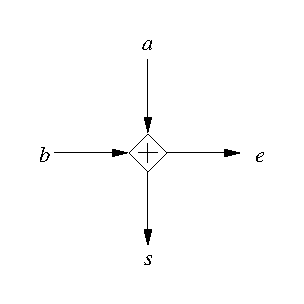
\includegraphics{quick-two-sum.eps}
      \caption{\label{quick_two_sum_fig}{\sc Quick-Two-Sum}}
    \end{center}
  \end{minipage}
  \begin{minipage}[t]{2in}
    \begin{center}
      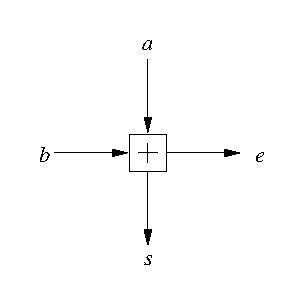
\includegraphics{two-sum.eps}
      \caption{\label{two_sum_fig}{\sc Two-Sum}}
    \end{center}
  \end{minipage}
  \begin{minipage}[t]{2in}
    \begin{center}
      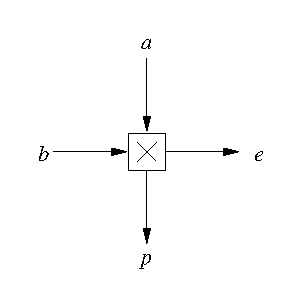
\includegraphics{two-prod.eps}
      \caption{\label{two_prod_fig}{\sc Two-Prod}}
    \end{center}
  \end{minipage}
\end{figure}

\begin{figure}
  \begin{center}
    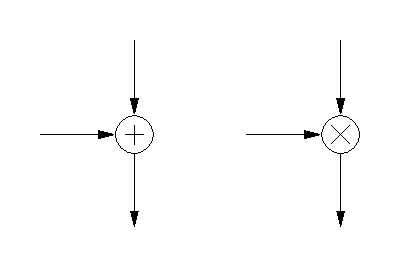
\includegraphics{normal_sum_prod.eps}
    \caption{\label{normal_sum_prod_fig}Normal IEEE double precision sum and product}
  \end{center}
\end{figure}

\section{Basic Operations} \label{sec:basic}
\subsection{Renormalization}
A quad-double number is an unevaluated sum of four IEEE double numbers.
The quad-double number $(a_0, a_1, a_2, a_3)$ represents the exact
sum $a = a_0 + a_1 + a_2 + a_3$.  Note that for any given representable
number $x$, there can be many representations as an unevaluated sum of
four doubles.  Hence we require that the quadruple $(a_0, a_1, a_2, a_3)$
to satisfy
\begin{displaymath}
  |a_{i+1}| \le \frac{1}{2}\ulp(a_i)  
\end{displaymath}
for $i = 0, 1, 2$, with equality occurring only if $a_i = 0$ or 
the last bit of $a_i$ is $0$ (that is, round-to-even is used in case
of ties).  Note that the first double $a_0$ is a double-precision
approximation to the quad-double number $a$, accurate to almost
half an ulp.

\begin{lem}
  For any quad-double number $a = (a_0, a_1, a_2, a_3)$, the normalized 
  representation is unique.
\end{lem}

Most of the algorithms described here produce an expansion that
is not of canonical form -- often having overlapping bits.  
Therefore, a five-term expansion is produced, and then renormalized
to four components.

\begin{alg}
  \label{renorm_alg}
  This renormalization procedure is a variant of Priest's renormalization
  method \cite[p. 116]{pri92}.  The input is a five-term expansion with 
  limited overlapping bits, with $a_0$ being the most significant component.  

  \vspace{0.1in} \hfill
  \begin{minipage}[t]{5in}
    {\sc Renormalize}($a_0, a_1, a_2, a_3, a_4$) \\
    \begin{tabular}{rl}
      1.  & $(s, t_4) \leftarrow$ {\sc Quick-Two-Sum}($a_3, a_4$) \\
      2.  & $(s, t_3) \leftarrow$ {\sc Quick-Two-Sum}($a_2, s$)   \\
      3.  & $(s, t_2) \leftarrow$ {\sc Quick-Two-Sum}($a_1, s$)   \\
      4.  & $(t_0, t_1) \leftarrow$ {\sc Quick-Two-Sum}($a_0, s$) \\
      \\
      5.  & $s \leftarrow t_0$ \\
      6.  & $k \leftarrow 0$   \\
      7.  & {\bf for\footnotemark[1]} $i \leftarrow 1, 2, 3, 4$ \\
      8.  & \quad $(s, e) \leftarrow$ {\sc Quick-Two-Sum}($s, t_i$) \\
      9.  & \quad {\bf if} $e \ne 0$             \\
      10. & \quad \quad $b_k \leftarrow s$       \\
      11. & \quad \quad $s \leftarrow e$         \\
      12. & \quad \quad $k \leftarrow k + 1$     \\
      13. & \quad {\bf end if}  \\
      14. & {\bf end for} \\
      15. & {\bf return} $(b_0, b_1, b_2, b_3)$
    \end{tabular}
  \end{minipage}  
\end{alg}

\footnotetext[1]{In the implementation, this loop is unrolled to several
  {\tt if} statements.}

Necessary conditions for this renormalization algorithm to work correctly
are, unfortunately, not known.  Priest proves that if the input expansion
does not overlap by more than 51 bits, then the algorithm works correctly.
However, this condition is by no means necessary; that the renormalization
algorithm (Algorithm \ref{renorm_alg})
works on all the expansions produced by the algorithms below 
remains to be shown.

\subsection{Addition}
\subsubsection{Quad-Double + Double}
The addition of a double precision number to a quad-double number
is similar to Shewchuk's {\sc Grow-Expansion} \cite[p. 316]{she97}, but the double 
precision number $b$ is added to a quad-double number $a$ from
most significant component first (rather than from least significant).
This produces a five-term expansion which is the exact result, 
which is then renormalized.  See Figure~\ref{qd_add_qd_d_fig}.

\begin{figure}
  \begin{center} 
    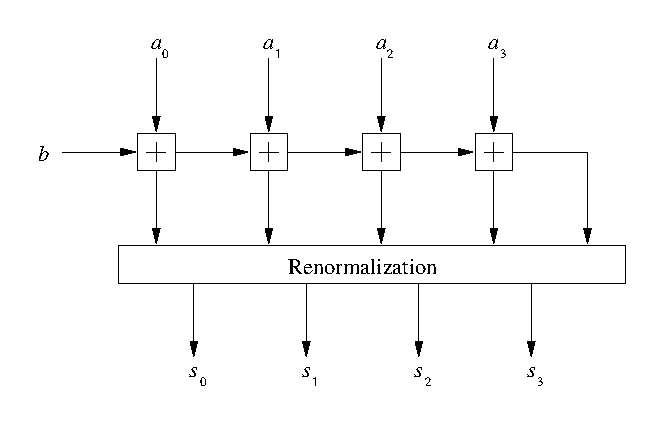
\includegraphics{qd_add_qd_d.eps}
    \caption{\label{qd_add_qd_d_fig}Quad-Double + Double}
  \end{center}
\end{figure}

Since the exact result is computed, then normalized to four components, 
this addition is accurate to at least the first 212 bits of the result.

\subsubsection{Quad-Double + Quad-Double}
We have implemented two algorithms for addition.  The first one
is faster, but only satisfies the weaker (Cray-style) error bound
$a \oplus b = (1 + \delta_1)a + (1 + \delta_2)b$ where the magnitude
of $\delta_1$ and $\delta_2$ is bounded by $\epsqd = 2^{-211}$.

\begin{figure}
  \begin{center} 
    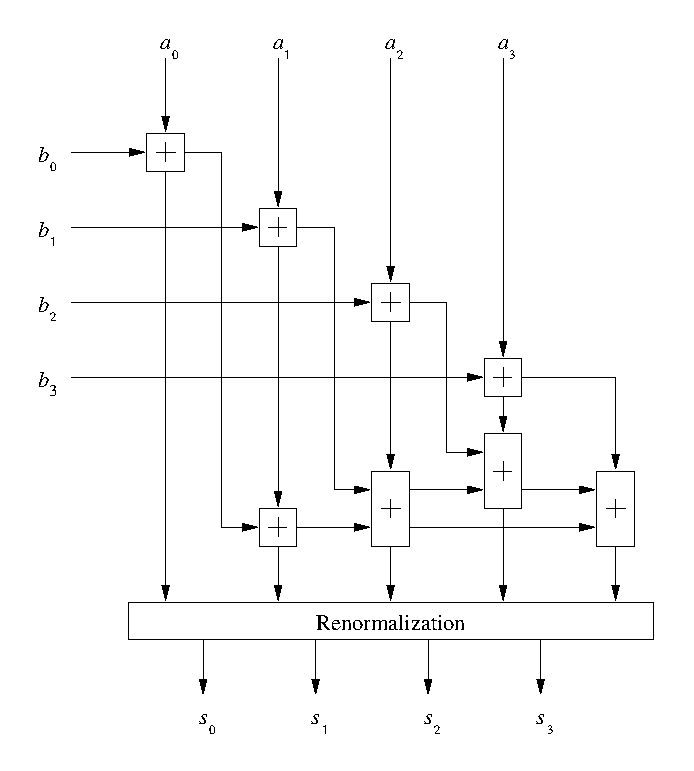
\includegraphics{qd_add.eps}
    \caption{\label{qd_add_fig}Quad-Double + Quad-Double}
  \end{center}
\end{figure}

Figure \ref{qd_add_fig} best describes the first addition algorithm of two
quad-double numbers.  In the diagram, there are three large boxes
with three inputs to them.  These are various {\sc Three-Sum} boxes, 
and their internals are shown in Figure \ref{three_sum_fig}.

\begin{figure}
  \begin{center}
    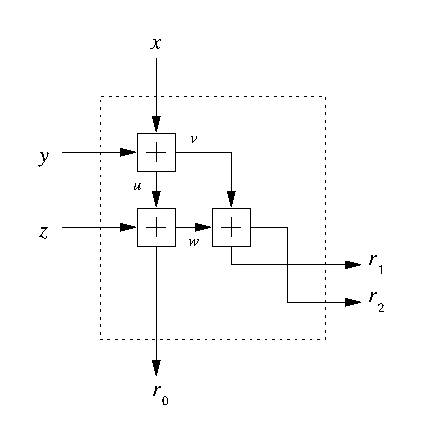
\includegraphics{three-sum.eps} 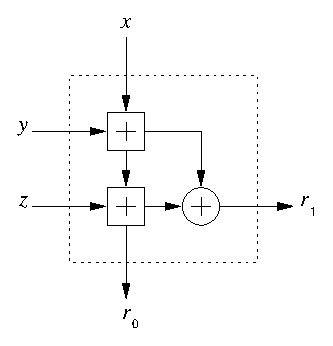
\includegraphics{three-sum-2.eps}
    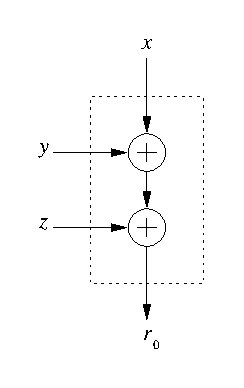
\includegraphics{three-sum-3.eps}
    \caption{\label{three_sum_fig}{\sc Three-Sum}s}
  \end{center}
\end{figure}

Now for a few more lemmas.
\begin{lem}
  \label{two_sum_bound}
  Let $a$ and $b$ be two double precision floating point numbers.
  Let $M = \max(|a|, |b|)$.  Then $|\fl(a+b)| \le 2M$, and consequently, 
  $|\err(a+b)| \le \frac{1}{2}\ulp(2M) \le 2 \eps M$.
\end{lem}

\begin{lem}
  \label{three_sum_bound}
  Let $x, y,$ and $z$ be inputs to {\sc Three-Sum}.
  Let $u, v, w, r_0, r_1,$ and $r_2$ be as indicated in Figure 
  \ref{three_sum_fig}.  Let $M = \max (|x|, |y|, |z|)$.  Then
  $|r_0| \le 4M$, $|r_1| \le 8 \eps M$, and $|r_2| \le 8 \eps^2 M$.
\end{lem}
\begin{proof} This follows from applying Lemma \ref{two_sum_bound}
to each of the three {\sc Two-Sum} boxes.  
First {\sc Two-Sum} gives $|u| \le 2M$ and
$|v| \le 2\eps M$.  Next {\sc Two-Sum} (adding $u$ and $z$) gives
$|r_0| \le 4M$ and $|w| \le 4\eps M$.  Finally, the last {\sc Two-Sum}
gives the desired result.
\end{proof}

Note that the two other {\sc Three-Sum}s shown are simplification
of the first {\sc Three-Sum}, where it only computes one or two components, 
instead of three; thus the same bounds apply.

The above bound is not at all tight; $|r_0|$ is bounded closer
to $3M$ (or even $|x| + |y| + |z|$), and this makes the bounds for $r_1$ 
and $r_2$ correspondingly smaller.  However, this suffices for the
following lemma.

\begin{lem}\label{sum_lemma}
  The five-term expansion before the renormalization step in the
  quad-double addition algorithm shown in Figure \ref{qd_add_fig} errs 
  from the true result by less than $\epsqd M$, where $M = \max(|a|, |b|)$.
\end{lem}
\begin{proof}
This can be shown by
judiciously applying Lemmas \ref{two_sum_bound} and \ref{three_sum_bound}
to all the {\sc Two-Sum}s and {\sc Three-Sum}s in Figure \ref{qd_add_fig}.
See Appendix \ref{proof_appendix} for detailed proof.
\end{proof}

Assuming that the renormalization
step works (this remains to be proven), we can then obtain the error bound
\begin{displaymath}
  \fl(a+b) = (1 + \delta_1) a + (1 + \delta_2) b \qquad \textrm{with} \quad
  |\delta_1|, |\delta_2| \le \epsqd.
\end{displaymath}

Note that the above algorithm for addition is particularly suited to 
modern processors with instruction level parallelism, since the first
four {\sc Two-Sum}s can be evaluated in parallel.  Lack of branches 
before the renormalization step also helps to keep the pipelines full.

Note that the above algorithm does not satisfy the IEEE-style error
bound 
\begin{displaymath}
  \fl(a+b) = (1+\delta)(a+b) \qquad \textrm{with} \quad
  |\delta| \le 2\epsqd \textrm{ or so.}
\end{displaymath}
To see this, let $a = (u, v, w, x)$ and $b = (-u, -v, y, z)$, 
where none of $w, x, y, z$ overlaps and $|w| > |x| > |y| > |z|$.
Then the above algorithm produces $c = (w, x, y, 0)$ instead
of $c = (w, x, y, z)$ required by the stricter bound.

The second algorithm, due to J. Shewchuk and S. Boldo, computes the first
four components of the {\em result} correctly.  Thus it satisfies
more strict error bound
\begin{displaymath}
  \fl(a+b) = (1+\delta)(a+b) \qquad \textrm{with} \quad
  |\delta| \le 2\epsqd \textrm{ or so.}
\end{displaymath}
However, it has a corresponding speed penalty; it runs significantly slower
(factor of $2$--$3.5$ slower).

The algorithm is similar to Shewchuk's {\sc Fast-Expansion-Sum} 
\cite[p. 320]{she97}, 
where it merge-sorts the two expansions.  To prevent components with
only a few significant bits to be produced, a double-length accumulator
is used so that a component is output only if the inputs gets small 
enough to not affect it.  

\begin{alg}
  \label{double_accum_alg}
  Assuming that $u, v$ is a two-term expansion, the following algorithm
  computes the sum $(u, v) + x$, and outputs the significant component
  $s$ if the remaining components contain more than one double worth
  of significand. $u$ and $v$ are modified to represent the other
  two components in the sum.

  \vspace{0.1in} \hfill
  \begin{minipage}[t]{5in}
    {\sc Double-Accumulate}($u, v, x$) \\
    \begin{tabular}{rl}
      1.  & $(s, v) \leftarrow$ {\sc Two-Sum}($v, x$)  \\
      2.  & $(s, u) \leftarrow$ {\sc Two-Sum}($u, s$)  \\
      3.  & {\bf if} $u = 0$ \\
      4.  & \quad $u \leftarrow s$ \\
      5.  & \quad $s \leftarrow 0$ \\
      6.  & {\bf end if} \\
      7.  & {\bf if} $v = 0$ \\
      8.  & \quad $v \leftarrow u$ \\
      9.  & \quad $u \leftarrow s$ \\
      10. & \quad $s \leftarrow 0$ \\
      11. & {\bf end if}   \\
      12. & {\bf return} ($s, u, v$) \\
    \end{tabular}
  \end{minipage}  
\end{alg}

The accurate addition scheme is given by the following algorithm.
\begin{alg}
  \label{accurate_add_alg}
  This algorithm computes the sum of two quad-double numbers 
  $a = (a_0, a_1, a_2, a_3)$ and $b = (b_0, b_1, b_2, b_3)$.
  Basically it merge-sorts the eight doubles, and performs
  {\sc Double-Accumulate} until four components are obtained.

  \vspace{0.1in} \hfill
  \begin{minipage}[t]{5in}
    {\sc QD-Add-Accurate}($a, b$) \\
    \begin{tabular}{rl}
      1.  & $(x_0, x_1, \ldots, x_7) \leftarrow$ 
          {\sc Merge-Sort}$(a_0, a_1, a_2, a_3, b_0, b_1, b_2, b_3)$ \\
      2.  & $u \leftarrow 0$ \\
      3.  & $v \leftarrow 0$ \\
      4.  & $k \leftarrow 0$ \\
      5.  & $i \leftarrow 0$ \\
      6.  & {\bf while} $k < 4$ {\bf and} $i < 8$ {\bf do} \\
      7.  & \quad $(s,u,v)\leftarrow$ {\sc Double-Accumulate}$(u, v, x_i)$ \\
      8.  & \quad {\bf if} $s \ne 0$ \\
      9.  & \quad \quad $c_k \leftarrow s$ \\
     10.  & \quad \quad $k \leftarrow k + 1$ \\
     11.  & \quad {\bf end if} \\
     12.  & \quad $i \leftarrow i + 1$ \\
     13.  & {\bf end while} \\
     14.  & {\bf if} $k < 2$ {\bf then} $c_{k+1} \leftarrow v$ \\
     15.  & {\bf if} $k < 3$ {\bf then} $c_k \leftarrow u$ \\
     16.  & {\bf return} {\sc Renormalize}$(c_0, c_1, c_2, c_3)$
    \end{tabular}
  \end{minipage}
\end{alg}

\subsection{Subtraction}
Subtraction $a - b$ is implemented as the addition $a + (-b)$, 
so it has the same algorithm and properties as that of addition.
To negate a quad-double number, we can just simply negate each component.
On a modern C++ compiler with inlining, the overhead is
noticeable but not prohibitive (say $5\%$ or so).

\subsection{Multiplication}
Multiplication is basically done in a straightforward way, multiplying
term by term and accumulating.  Note that unlike addition, there
are no possibilities of massive cancellation in multiplication, so
the following algorithms satisfy the IEEE style error bound
$a \otimes b = (1 + \delta)(a \times b)$ where $\delta$ is bounded
by $\epsqd$.

\subsubsection{Quad-Double $\times$ Double}
Let $a = (a_0, a_1, a_2, a_3)$ be a quad-double number, and let $b$ be
a double precision number.  Then the product is the sum of four terms, 
$a_0 b + a_1 b + a_2 b + a_3 b$.  Note that $|a_3| \le \eps^3 |a_0|$, 
so $|a_3 b| \le \eps^3 |a_0 b|$, and thus only the first 53 bits of
the product $a_3 b$ need to be computed.  The first three terms are
computed exactly using {\sc Two-Prod} (or {\sc Two-Prod-FMA}).
All the terms are then accumulated in a similar fashion as addition.
See Figure \ref{qd_mul_qd_d_fig}.

\begin{figure}
  \begin{center} 
    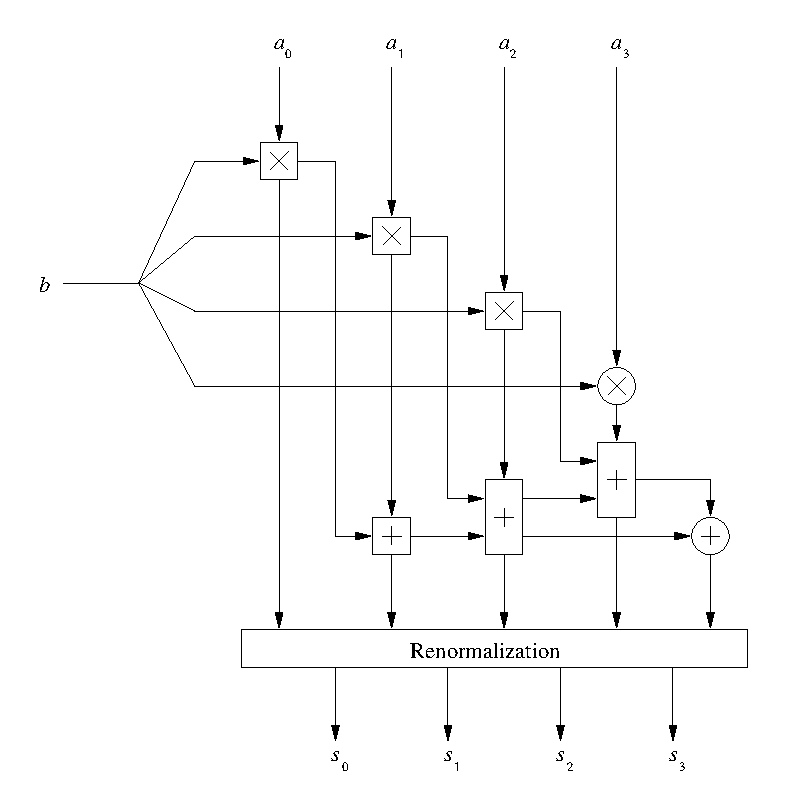
\includegraphics{qd_mul_qd_d.eps}
    \caption{\label{qd_mul_qd_d_fig}Quad-Double $\times$ Double}
  \end{center}
\end{figure}

\subsubsection{Quad-Double $\times$ Quad-Double}
Multiplication of two quad-double numbers becomes a bit complicated, 
but nevertheless follows the same idea.  Let $a = (a_0, a_1, a_2, a_3)$
and $b = (b_0, b_1, b_2, b_3)$ be two quad-double numbers.  Assume
(without loss of generality) that $a$ and $b$ are order 1.
After multiplication, we need to accumulate $13$ terms of order $O(\eps^4)$
or higher.
\begin{displaymath}
  \begin{array}{rcl@{\qquad}l}
    a \times b &\approx& a_0 b_0 & O(1) \textrm{ term} \\
    & & +\; a_0 b_1 + a_1 b_0 & O(\eps) \textrm{ terms}\\
    & & +\;a_0 b_2 + a_1 b_1 + a_2 b_0 & O(\eps^2) \textrm{ terms}\\
    & & +\;a_0 b_3 + a_1 b_2 + a_2 b_1 + a_3 b_0 & O(\eps^3) \textrm{ terms}\\
    & & +\;a_1 b_3 + a_2 b_2 + a_3 b_1 & O(\eps^4) \textrm{ terms}
  \end{array}
\end{displaymath}
Note that smaller order terms (such as $a_2 b_3$, which is $O(\eps^5)$)
are not even computed, since they are not needed to get the first
212 bits.  The $O(\eps^4)$ terms are computed using normal double
precision arithmetic, as only their first few bits are needed.

For $i+j \le 3$, let $(p_{ij}, q_{ij}) = ${\sc Two-Prod}($a_i$, $b_j$).  
Then $p_{ij} = O(\eps^{i+j})$ and $q_{ij} = O(\eps^{i+j+1})$.
Now there are one term ($p_{00}$) of order $O(1)$, three 
($p_{01}$, $p_{10}$, $q_{00}$) of order $O(\eps)$, five 
($p_{02}$, $p_{11}$, $p_{20}$, $q_{01}$, $q_{10}$) 
of order $O(\eps^2)$, seven of order $O(\eps^3)$, 
and seven of order $O(\eps^4)$.
Now we can start accumulating all the terms by their order, 
starting with $O(\eps)$ terms (see Figure \ref{qd_mul_accum_fig}).

\begin{figure}
  \begin{center} 
    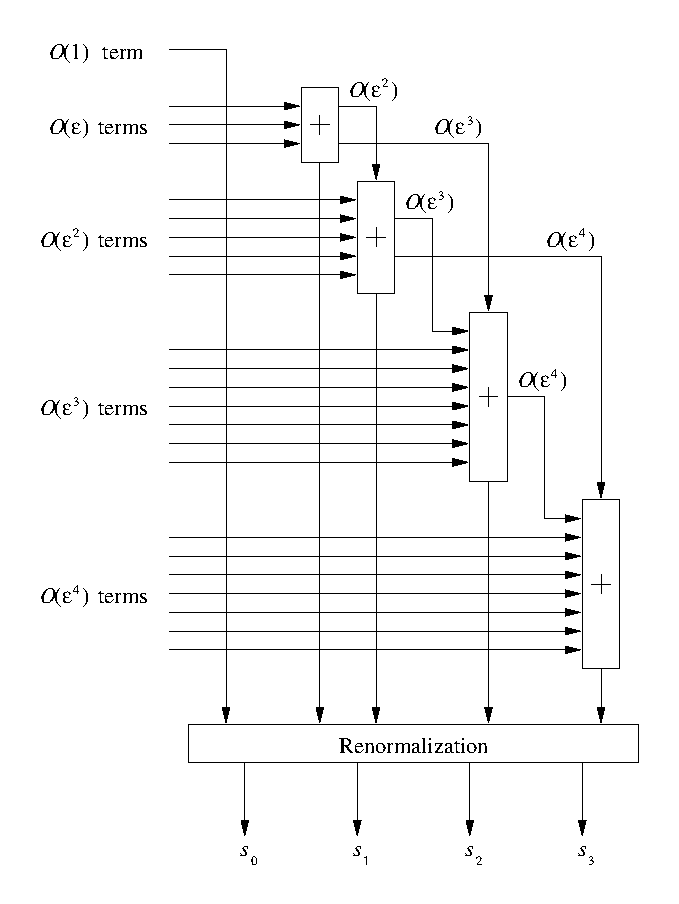
\includegraphics{qd_mul_accum.eps}
    \caption{\label{qd_mul_accum_fig}Quad-Double $\times$ Quad-Double accumulation phase}
  \end{center}
\end{figure}

In the diagram, there are four different summation boxes.
The first (topmost) one is {\sc Three-Sum}, same as the one in 
addition.  The next three are, respectively, {\sc Six-Three-Sum}
(sums six doubles and outputs the first three components), 
{\sc Nine-Two-Sum} (sums nine doubles and outputs the first two components), 
and {\sc Nine-One-Sum} (just adds nine doubles using normal arithmetic).

{\sc Six-Three-Sum} computes the sum of six doubles to three double
worth of accuracy (i.e., to relative error of $O(\eps^3)$).  This is
done by dividing the inputs into two groups of three, and 
performing {\sc Three-Sum} on each group.  Then the two sums
are added together, in a manner similar to quad-double addition.
See Figure \ref{six_three_sum_fig}.

{\sc Nine-Two-Sum} computes the sum of nine doubles to double-double
accuracy.  This is done by pairing the inputs to create four double-double
numbers and a single double precision number, and performing
addition of two double-double numbers recursively until one arrives
at a double-double output.  The double-double addition (the large square
box in the diagram) is the same as David Bailey's algorithm \cite{bai-dd}.
See Figure \ref{nine_two_sum_fig}.

\begin{figure}
  \begin{center} 
    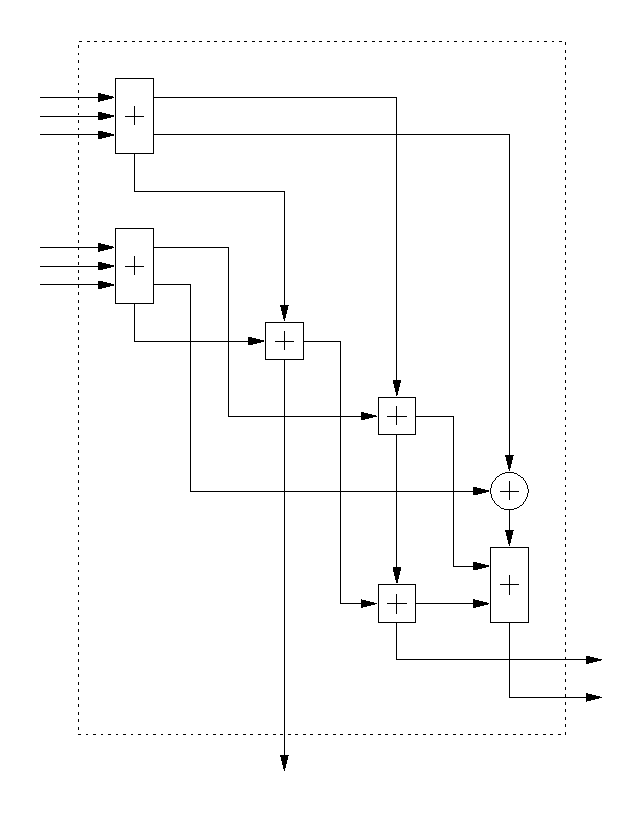
\includegraphics{six-three-sum.eps}
    \caption{\label{six_three_sum_fig}{\sc Six-Three-Sum}}
  \end{center}
\end{figure}

\begin{figure}
  \begin{center} 
    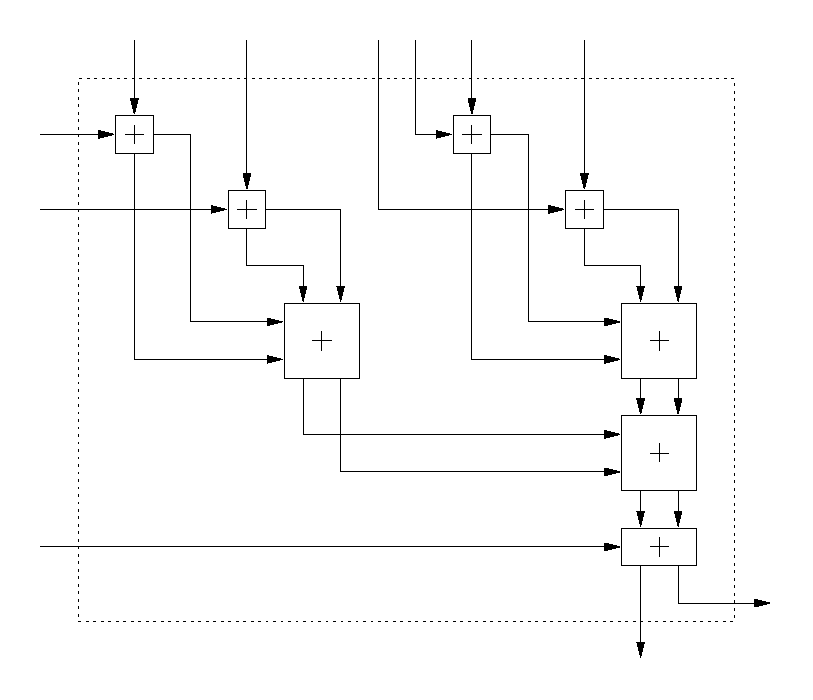
\includegraphics{nine-two-sum.eps}
    \caption{\label{nine_two_sum_fig}{\sc Nine-Two-Sum}}
  \end{center}
\end{figure}

If one wishes to trade few bits of accuracy for speed, we don't
even need to compute the $O(\eps^4)$ terms; they can affect the
first 212 bits only by carries during accumulation.  
In this case, we can compute the
$O(\eps^3)$ terms using normal double precision arithmetic, 
thereby speeding up multiplication considerably.

Squaring a quad-double number can be done significantly
faster since the number of terms that needs to be accumulated
can be reduced due to symmetry.

\subsection{Division}
Division is done by the familiar long division algorithm.
Let $a = (a_0, a_1, a_2, a_3)$ and $b = (b_0, b_1, b_2, b_3)$ be 
quad-double numbers.  We can first compute
an approximate quotient $q_0 = a_0 / b_0$.  We then compute
the remainder $r = a - q_0 \times b$, and compute the 
correction term $q_1 = r_0 / b_0$.  We can continue this process 
to obtain five terms, $q_0,\; q_1,\; q_2,\; q_3$, and $q_4$.
(only four are needed if few bits of accuracy is not important).

Note that at each step, full quad-double multiplication and 
subtraction must be done since most of the bits will be canceled
when computing $q_3$ and $q_4$.  The five-term (or four-term)
expansion is then renormalized to obtain the quad-double quotient.

\section{Algebraic Operations} \label{sec:algebraic}
\subsection{$N$-th Power}
$N$-th Power computes $a^n$, given a quad-double number $a$ and an
integer $n$.  This is simply done by repeated squaring, borrowed
from David Bailey \cite{bai-dd}. 

\subsection{Square Root}
Square root computes $\sqrt{a}$ given a quad-double number $a$.
This is done with Newton iteration on the function
\begin{displaymath}
  f(x) = \frac{1}{x^2} - a
\end{displaymath}
which has the roots $\pm a^{-1/2}$. This gives rise to the iteration
\begin{displaymath}
  x_{i+1} = x_i + \frac{x_i (1 - ax_i^2)}{2}.
\end{displaymath}
Note that the iteration does not require division of quad-double
numbers.  (Multiplication by $1/2$ can be done component-wise.)
Since Newton's iteration is locally quadratically convergent, 
only about two iterations are required if one starts out with
double precision approximation $x_0 = \sqrt{a_0}$.  (In the
implementation it is done three times.)  After $x = a^{-1/2}$ is
computed, we perform a multiplication to obtain $\sqrt{a} = ax$.

\subsection{$N$-th Root}
$N$-th Root computes $\sqrt[n]{a}$ given a quad-double number $a$
and an integer $n$.  This is done again by Newton's iteration on
the function
\begin{displaymath}
  f(x) = \frac{1}{x^n} - a
\end{displaymath}
which has the roots $a^{-1/n}$. This gives rise to the iteration
\begin{displaymath}
  x_{i+1} = x_i + \frac{x_i (1 - ax_i^n)}{n}.
\end{displaymath}
Three iterations are performed, although twice is almost sufficient.
After $x = a^{-1/n}$ is computed, we can invert to obtain $a^{1/n} = 1/x$.

\section{Transcendental Operations} \label{sec:transcendental}
\subsection{Exponential}
The classic Taylor-Maclaurin series is used to evaluate $e^x$.  Before
using the Taylor series, the argument is reduced by noting that
\begin{displaymath}
  e^{kr + m \log 2} = 2^m (e^r)^k, 
\end{displaymath}
where the integer $m$ is chosen so that $m \log 2$ is closest to $x$.
This way, we can make $|kr| \le \frac{1}{2} \log 2 \approx 0.34657$.
Using $k = 256$, we have $|r| \le \frac{1}{512} \log 2 \approx 0.001354$.
Now $e^r$ can be evaluated using familiar Taylor series.  The argument
reduction substantially speeds up the convergence of the series, as
at most 18 terms are need to be added in the Taylor series.

\subsection{Logarithm}
Since the Taylor series for logarithm converges much more slowly than 
the series for exponential, instead we use Newton's iteration to
find the zero of the function $f(x) = e^x - a$.  This leads to 
the iteration
\begin{displaymath}
  x_{i+1} = x_i + ae^{-x_i} - 1, 
\end{displaymath}
which is repeated three times.

\subsection{Trigonometrics}
Sine and cosine are computed using Taylor series after argument reduction.
To compute $\sin x$ and $\cos x$, the argument $x$ is first reduced modulo
$2 \pi$, so that $|x| \le \pi$.  Now noting that $\sin (y + k \pi /2)$
and $\cos (y + k \pi / 2)$ are of the form $\pm \sin y$ or $\pm \cos y$
for all integers $k$, we can reduce the argument modulo $\pi/2$ so that
we only need to compute $\sin y$ and $\cos y$ with $|y| \le \pi / 4$.

Finally, write $y = z + m (\pi / 1024)$ where the integer $m$ is chosen
so that $|z| \le \pi / 2048 \approx 0.001534$.  Since $|y| \le \pi / 4$, 
we can assume that $|m| \le 256$.
By using a precomputed table
of $\sin (m \pi / 1024)$ and $\cos (m \pi / 1024)$, we note that
\begin{displaymath}
  \sin (z + m \pi / 1024) = \sin z \cos (m \pi / 1024) + 
  \cos z \sin (m \pi / 1024)
\end{displaymath}
and similarly for $\cos (z + m \pi / 1024)$.  Using this argument
reduction significantly increases the convergence rate of sine, 
as at most 10 terms need be added.

Note that if both cosine and sine are needed, then one can compute
the cosine using the formula 
\begin{displaymath}
  \cos x = \sqrt{1 - \sin^2 x}.
\end{displaymath}

The values of $\sin (m \pi / 1024)$ and $\cos (m \pi / 1024)$ are
precomputed by using arbitrary precision package such as MPFUN \cite{bai-mp}
using the formula
\begin{displaymath}
    \sin \left( \frac{\theta}{2} \right) = 
    \frac{1}{2} \sqrt{2 - 2 \cos \theta}
\end{displaymath}
\begin{displaymath}
    \cos \left( \frac{\theta}{2} \right) = 
    \frac{1}{2} \sqrt{2 + 2 \cos \theta}
\end{displaymath}
Starting with $\cos \pi = -1$, we can recursively use the above formula
to obtain $\sin (m \pi / 1024)$ and $\cos (m \pi / 1024)$.

\subsection{Inverse Trigonometrics}
Inverse trigonometric function $\arctan$ is computed using Newton
iteration on the function $f(x) = \sin x - a$.

\subsection{Hyperbolic Functions}
Hyperbolic sine and cosine are computed using
\begin{displaymath} 
  \sinh x = \frac{e^x - e^{-x}}{2} \qquad \cosh x = \frac{e^x + e^{-x}}{2}
\end{displaymath}
However, when $x$ is small (say $|x| \le 0.01$), the above formula for 
$\sinh$ becomes unstable, and the Taylor series is used instead.

\section{Miscellaneous Routines} \label{sec:misc}
\subsection{Input / Output}
  Binary to decimal conversion of quad-double number $x$ is done by 
determining the integer $k$ such that $1 \le |x 10^{-k}| < 10$, 
and repeatedly extracting digits and multiplying by 10.  To minimize
error accumulation, a table of accurately precomputed powers of 10
is used.  This table is also used in decimal to binary conversion.

\subsection{Comparisons}
Since quad-double numbers are fully renormalized after each 
operation, comparing two quad-double number for equality can
be done component-wise.  Comparing the size can be done from
most significant component first, similar to dictionary ordering
of English words.  Comparison to zero can be done just by checking
the most significant word.

\subsection{Random Number Generator}
The quad-double random number generator produces a quad-double
number in the range $[0, 1)$, uniformly distributed.  This is 
done by choosing the first 212 bits randomly.  A 31-bit system-supplied
random number generator is used to generate 31 bits at a time, 
this is repeated $\lceil 212 / 31 \rceil = 7$ times to get
all 212 bits.

\section{C++ Implementation} \label{sec:implement}
  The quad-double library is implemented in ANSI C++, taking full
advantage of operator / function overloading and user-defined data 
structures.  The library should compile fine with ANSI Standard compliant
C++ compilers.  Some of the test codes may not work with compilers
lacking full support for templates.  Please see the files {\tt README}
and {\tt INSTALL} for more details on the implementation and build 
instructions.

  Full C++ implementation of double-double library is included as
a part of the quad-double library, including full support for mixing
three types: double, double-double, and quad-double.  In order to use
the library, one must include the header file {\tt qd.h} 
and link the code with the library {\tt libqd.a}.  
Quad-double variables are declared as {\tt qd\_real}, while double-double
variables are declared as {\tt dd\_real}.

A sample C++ program is given below.

\bigskip

\begin{minipage}{0.8\textwidth}
\begin{tt}\begin{verbatim}
  #include <iostream>
  #include <qd/qd_real.h>

  using std::cout;
  using std::endl;

  int main() {
    unsigned int oldcw;
    fpu_fix_start(&oldcw);     // see notes on x86 machines below.

    qd_real a = "3.141592653589793238462643383279502884197169399375105820";
    dd_real b = "2.249775724709369995957";
    qd_real r;
    
    r = sqrt(a * b + 1.0);
    cout << " sqrt(a * b + 1) = " << r << endl;

    fpu_fix_end(&oldcw);       // see notes on x86 machines below.
    return 0;
  }
\end{verbatim}\end{tt}
\end{minipage}

\bigskip

Note that strings must be used to assign to a quad-double (or double-double)
numbers; otherwise the double precision approximation is assigned.
For example, {\tt a = 0.1} does not assign quad-double precision 0.1, 
but rather a double precision number 0.1.  Instead, use {\tt a = "0.1"}.

Common constants such as $\pi$, $\pi/2$, $\pi/4$, $e$, $\log 2$ are
 provided as {\tt qd\_real::\_pi}, {\tt qd\_real::\_pi2}, 
{\tt qd\_real::\_pi4}, {\tt qd\_real::\_e}, and {\tt qd\_real::\_log2}.
These were computed using an arbitrary precision package (MPFUN++ 
\cite{cha98}), and therefore are accurate to the last bit.

\noindent{\bf Note on Intel x86 Processors}.
The algorithms in this library assume IEEE double precision floating
point arithmetic.  Since Intel x86 processors have extended (80-bit)
floating point registers, the round-to-double flag must be enabled in
the control word of the FPU for this library to function properly
under x86 processors.  The function {\tt fpu\_fix\_start} turns
on the round-to-double bit in the FPU control word, while 
{\tt fpu\_fix\_end} will restore the original state.

\section{Performance} \label{sec:performance}
Performance of various operations on quad-double numbers on a variety
of machines are presented in Table \ref{timing_table}.  The tested
machines are
\begin{itemize}
\item Intel Pentium II, 400 MHz, Linux 2.2.16, g++ 2.95.2 compiler, 
  with {\tt -O3 -funroll-loops -finline-functions -mcpu=i686 -march=i686} 
  optimizations.
\item Sun UltraSparc 333 MHz, SunOS 5.7, Sun CC 5.0 compiler, 
  with {\tt -xO5 -native} optimizations.
\item PowerPC 750 (Apple G3), 266 MHz, Linux 2.2.15, g++ 2.95.2 compiler, 
  with {\tt -O3 -funroll-\\loops -finline-functions} optimizations.
\item IBM RS/6000 Power3, 200 MHz, AIX 3.4, IBM xlC compiler, 
  with {\tt -O3 -qarch=pwr3 -qtune\\=pwr3 -qstrict} optimizations.
\end{itemize}

\noindent {\bf Note}: For some reason, GNU C++ compiler ({\tt g++}) has
a terrible time optimizing the code for multiplication; it runs more than
15 times slower than the code compiled by Sun's CC compiler.

\begin{table}[t]
  \begin{center}
  \label{timing_table}
  \begin{tabular}{|l|c|c|c|c|} \hline
    Operation & 
    \begin{tabular}{c}Pentium II \\ 400MHz \\ Linux 2.2.16 \end{tabular} & 
    \begin{tabular}{c}UltraSparc \\ 333 MHz \\ SunOS 5.7 \end{tabular} & 
    \begin{tabular}{c}PowerPC 750 \\ 266 MHz \\ Linux 2.2.15 \end{tabular} & 
    \begin{tabular}{c}Power3 \\  200 MHz \\ AIX 3.4 \end{tabular} \\
    \hline
    \multicolumn{5}{|l|}{{\em Quad-double}} \\ 
    add          &  0.583 &  0.580 &  0.868 &  0.710 \\
    accurate add &  1.280 &  2.464 &  2.468 &  1.551 \\
    mul          &  1.965 &  1.153 &  1.744 &  1.131 \\
    sloppy mul   &  1.016 &  0.860 &  1.177 &  0.875 \\
    div          &  5.267 &  6.440 &  8.210 &  6.699 \\
    sloppy div   &  4.080 &  4.163 &  6.200 &  4.979 \\
    sqrt         & 23.646 & 15.003 & 21.415 & 16.174 \\ \hline
    \multicolumn{5}{|l|}{{\em MPFUN}}\\
    add		 &  5.729 &  5.362 &  ---   &  4.651 \\
    mul		 &  7.624 &  7.630 &  ---   &  5.837 \\
    div     	 & 10.102 & 10.164 &  ---   &  9.180 \\ \hline
  \end{tabular}
  \caption{Performance of some Quad-Double algorithms on several machines. 
    All measurements are in microseconds. We include the performance of 
    MPFUN~\cite{bai-mp} as a comparison. Note, we do not have the MPFUN
    measurements on the PowerPC, because we do not have a Fortran-90 compiler.}
  \end{center}
\end{table}

Most of the routines runs noticeably faster if implemented in C, 
it seems that C++ operator overloading has some overhead associated
with it -- most notably excessive copying of quad-double numbers.
This occurs because operator overloading does not account for
where the result is going to be placed.  For example, 
for the code 
\begin{quote}\begin{tt}c = a + b;\end{tt}\end{quote}
the C++ compiler often emits the code equivalent to
\begin{quote}\begin{tt}
\begin{verbatim}
qd_real temp;
temp = operator+(a, b);     // Addition
operator=(c, temp);         // Copy result to c
\end{verbatim}
\end{tt}\end{quote}
In C, this copying does not happen, as one would just write
\begin{quote}\begin{tt}\begin{verbatim}
c_qd_add(a, b, c);          // Put (a+b) into c
\end{verbatim}\end{tt}\end{quote}
where the addition routine knows where to put the result directly.
This problem is somewhat alleviated by inlining, but not completely
eliminated.  There are techniques to avoid these kinds of copying~\cite{c++}, 
but they have
their own overheads associated with them and is not practical for
quad-double with only 32 bytes of data\footnote{These techniques
are feasible, for larger data structures, such as for much higher
precision arithmetics, where copying of data becomes time consuming.}.

\section{Future Work} \label{sec:future}
Currently, the basic routines do not have a full correctness proof.
The correctness of these routines rely on the fact that renormalization
step works; Priest proves that it does work if the input does not overlap
by 51 bits and no three components overlap at a single bit.  Whether
such overlap can occur in any of these algorithm needs to be proved.

There are improvements due in the remainder operator, which computes
$a - \round(a/b) \times b$, given quad-double numbers $a$ and $b$.
Currently, the library does the na\"\i ve method of just divide, round, 
multiply, and subtract.  This leads to loss of accuracy when $a$ is large
compared to $b$.  Since this routine is used in argument reduction for
exponentials, logarithms and trigonometrics, a fix is needed.

A natural extention of this work is to extend the precision beyond
quad-double.  Algorithms for quad-double additions and multiplication
can be extended to higher precisions, however, with more components, 
asymptotically faster algorithm due to S. Boldo and J. Shewchuk may
be preferrable (i.e. Algorithm~\ref{accurate_add_alg}).
One limitation these higher precision expansions have
is the limited exponent range -- same as that of double.  Hence 
the maximum precision is about 2000 bits (39 components), 
and this occurs only if the first component is near overflow and the 
last near underflow.

\section{Acknowledgements}
We thank Jonathan Shewchuk, 
Sylvie Boldo, and James Demmel for constructive discussions on 
various basic algorithms.  In particular, the accurate version of 
addition algorithm is due to S. Boldo and J. Shewchuk.  Problems with
remainder was pointed out by J.Demmel.

\appendix
\newpage
\section{Proof of Quad-Double Addition Error Bound (Lemma \ref{sum_lemma})}
\label{proof_appendix}

\noindent
{\bf Lemma \ref{sum_lemma}}. 
\emph{The five-term expansion before the renormalization step in the
quad-double addition algorithm shown in Figure \ref{qd_add_fig} errs 
from the true result by less than $\epsqd M$, where $M = \max(|a|, |b|)$.}

\begin{proof}
  The proof is done by applying Lemmas \ref{two_sum_bound} and 
\ref{three_sum_bound} to each of {\sc Two-Sum}s and {\sc Three-Sum}s.
Let $e_0, e_1, e_2, e_3, t_1, t_2, t_3, x_0, x_1, x_2, x_3, x_4, u, v, 
w, z, f_1, f_2$, and $f_3$ be as shown in Figure \ref{qd_add_proof_fig}.

We need to show
that the five-term expansion $(x_0, x_1, x_2, x_3, x_4)$ errs from the
true result by less than $\epsqd M$, where $M = \max(|a_0|, |b_0|)$.
Note that the only place that any error is introduced is in {\sc Three-Sum} 7
and {\sc Three-Sum} 8, where lower order terms $f_1, f_2,$ and $f_3$ are discarded.  
Hence it suffices to show $|f_1| + |f_2| + |f_3| \le \epsqd M$.

\begin{figure}[h]
  \begin{center} 
    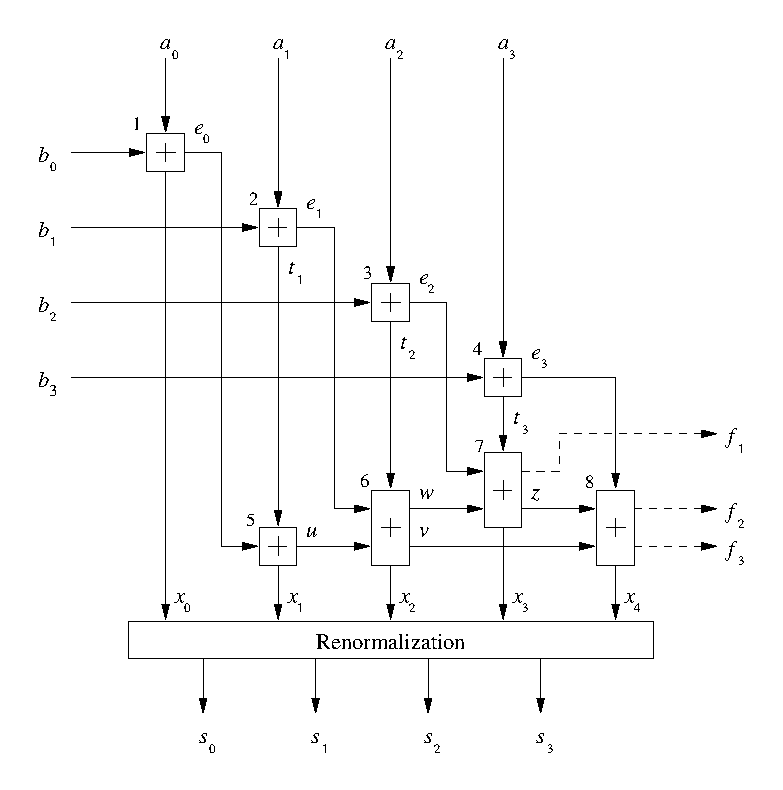
\includegraphics{qd_add_proof.eps}
    \caption{\label{qd_add_proof_fig}Quad-Double + Quad-Double}
  \end{center}
\end{figure}

First note that $|a_1| \le \eps M$, $|a_2| \le \eps^2 M$,and 
$|a_3| \le \eps^3 M$, since the input expansions are assumed to be 
normalized.  Similar inequalities applies for expansion $b$.
Applying Lemma \ref{two_sum_bound} to {\sc Two-Sum}s 1, 2, 3, 4, we obtain
\begin{displaymath}
  \begin{array}{rcl@{\qquad}rcl}
    |x_0| &\le& 2M & |e_0| &\le& 2\eps M\\
    |t_1| &\le& 2\eps M   & |e_1| &\le& 2\eps^2 M\\
    |t_2| &\le& 2\eps^2 M & |e_2| &\le& 2\eps^3 M\\
    |t_3| &\le& 2\eps^3 M & |e_3| &\le& 2\eps^4 M.
  \end{array}
\end{displaymath}

Now we can apply Lemma \ref{two_sum_bound} to {\sc Two-Sum} 5, to obtain
$|x_1| \le 4\eps M$ and $|u| \le 4 \eps^2 M$.  Then we apply Lemma 
\ref{three_sum_bound} to {\sc Three-Sum} 6 to obtain
\begin{displaymath}
  \begin{array}{r@{\;\le\;}l}
    |x_2| & 16\eps^2 M \\
    |w| & 32 \eps^3 M  \\
    |v| & 32 \eps^4 M.
  \end{array}
\end{displaymath}

Applying Lemma \ref{three_sum_bound} to {\sc Three-Sum} 7, we have
\begin{displaymath}
  \begin{array}{r@{\;\le\;}l}
    |x_3| & 128\eps^3 M \\
    |z| & 256 \eps^4 M  \\
    |f_1| & 256 \eps^5 M.
  \end{array}
\end{displaymath}

Finally we apply Lemma \ref{three_sum_bound} again to {\sc Three-Sum} 8
to get
\begin{displaymath}
  \begin{array}{r@{\;\le\;}l}
    |x_4| & 1024\eps^4 M \\
    |f_2| & 2048 \eps^5 M  \\
    |f_3| & 2048 \eps^6 M.
  \end{array}
\end{displaymath}

Thus we have 
\begin{displaymath}
  |f_1| + |f_2| + |f_3| \le 256 \eps^5 M + 2048 \eps^5 M + 2048 \eps^6 M 
  \le 2305 \eps^5 M \le \epsqd M
\end{displaymath}
as claimed.
\end{proof}

\newpage
\bibliographystyle{plain}
\bibliography{qd}

\end{document}
